% =====================================================================
% Figure: Parallel development timeline of TDA and CI with bridges
% Working draft -- user will refine final visual styling.
% =====================================================================
\begin{figure}[t]
\centering
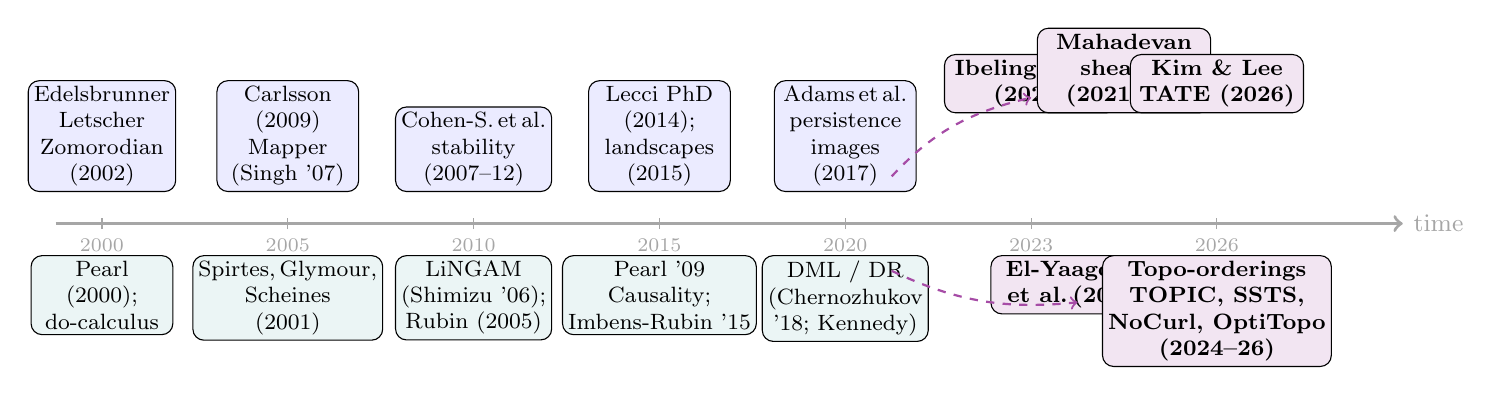
\begin{tikzpicture}[font=\footnotesize,
    yearnode/.style={draw, rounded corners, fill=blue!8, inner sep=2pt,
                     minimum width=18mm, align=center},
    cinode/.style={draw, rounded corners, fill=teal!8, inner sep=2pt,
                   minimum width=18mm, align=center},
    bridge/.style={draw, rounded corners, fill=violet!10, inner sep=2pt,
                   minimum width=22mm, align=center, font=\footnotesize\bfseries},
    xscale=1.18]
\draw[->, very thick, gray!70] (-0.5, 0) -- (14, 0)
  node[right, font=\small] {time};
\foreach \x/\y in {0/2000,2/2005,4/2010,6/2015,8/2020,10/2023,12/2026}{
  \draw[gray!70] (\x,-2pt) -- (\x,2pt) node[below=4pt, font=\scriptsize] {\y};
}
\node[yearnode, anchor=south] at (0,0.4)
  {Edelsbrunner\\Letscher\\Zomorodian\\(2002)};
\node[yearnode, anchor=south] at (2,0.4)
  {Carlsson\\(2009)\\Mapper\\(Singh '07)};
\node[yearnode, anchor=south] at (4,0.4)
  {Cohen-S.\,et\,al.\\stability\\(2007--12)};
\node[yearnode, anchor=south] at (6,0.4)
  {Lecci PhD\\(2014);\\landscapes\\(2015)};
\node[yearnode, anchor=south] at (8,0.4)
  {Adams\,et\,al.\\persistence\\images\\(2017)};

\node[cinode, anchor=north] at (0,-0.4)
  {Pearl\\(2000);\\do-calculus};
\node[cinode, anchor=north] at (2,-0.4)
  {Spirtes,\,Glymour,\\Scheines\\(2001)};
\node[cinode, anchor=north] at (4,-0.4)
  {LiNGAM\\(Shimizu '06);\\Rubin (2005)};
\node[cinode, anchor=north] at (6,-0.4)
  {Pearl '09\\Causality;\\Imbens-Rubin '15};
\node[cinode, anchor=north] at (8,-0.4)
  {DML / DR\\(Chernozhukov\\'18; Kennedy)};

\node[bridge, anchor=south] at (10,1.4)
  {Ibeling-Icard\\(2021)};
\node[bridge, anchor=south] at (11,1.4)
  {Mahadevan\\sheaves\\(2021--25)};
\node[bridge, anchor=south] at (12,1.4)
  {Kim \& Lee\\TATE (2026)};
\node[bridge, anchor=north] at (10.5,-0.4)
  {El-Yaagoubi\\et al.\,(2023)};
\node[bridge, anchor=north] at (12,-0.4)
  {Topo-orderings\\TOPIC, SSTS,\\NoCurl, OptiTopo\\(2024--26)};

\draw[->, dashed, thick, violet!70] (8.5,0.6) to[bend left=18] (10,1.6);
\draw[->, dashed, thick, violet!70] (8.5,-0.6) to[bend right=18] (10.5,-1.0);
\end{tikzpicture}
\caption{Parallel development of TDA (upper band, blue) and causal
inference (lower band, teal) with emerging bridges (violet) in the
2020s. Until $\sim$2020 the two communities developed largely
independently---TDA building from persistence and stability towards a
statistical-inference programme \citep{edelsbrunner2002topological,
carlsson2009topology,cohen2007stability,lecci2014statistical,
adams2017persistence}, while causal inference matured under the Pearl
and Rubin programmes and absorbed double-machine-learning
\citep{pearl2009causality,imbens2015causal,chernozhukov2018double}.
The bridge papers of 2021--2026---topology on the space of SCMs
\citep{ibeling2021topological}, sheaf-theoretic causal calculi
\citep{mahadevan2025sheaf}, topological treatment effects
\citep{kim2026topological}, simulation-based TDA inference for
multivariate time series \citep{elyaagoubi2023statistical}, and
topological-ordering algorithms for causal discovery
\citep{tran2024constraining,xu2025information,nocurl2024,
wu2026optimization}---together delineate the TCDA programme.}
\label{fig:timeline}
\end{figure}
